\documentclass{article}
\usepackage[utf8]{inputenc}
\usepackage{cancel}
\usepackage{amsthm,amssymb,amsmath}
\usepackage{mathtools}
\usepackage{tikz}
% in preamble
\usepackage{movie15}
% in documenet
\usepackage{fouriernc}
\usepackage{tkz-euclide}
\usetikzlibrary{calc, backgrounds}
\usepackage{tikz-3dplot}
\usetikzlibrary{positioning}
\usepackage{parskip}
\usepackage{float}
\tdplotsetmaincoords{70}{0}%
\newtheorem{theorem}{Theorem}[section]
\newtheorem{corollary}{Corollary}[theorem]
\newtheorem{lemma}[theorem]{Lemma}
\setlength{\parskip}{1em}
\newcommand{\NN}{\mathbb{N}}
\newcommand{\ZZ}{\mathbb{Z}}
\newcommand{\RR}{\mathbb{R}}
\newcommand{\QQ}{\mathbb{Q}}
\newcommand{\CC}{\mathbb{C}}
\newcommand{\xk}[1]{\vec{x}^{(#1)}}
\tdplotsetmaincoords{60}{110}
\def\r{{2*sqrt(3)}}
\title{MAT 4800 Homework \# 7 }
\author{Noah Reef }
\date{Spring 2023}

\usepackage{natbib}
\usepackage{graphicx}

\begin{document}
\maketitle

\section*{Problem \#1}
Suppose we are given the following function,

\begin{equation*}
    f(x_1,x_2) = 2x_1^4 + x_2^2 -4x_1x_2 + 5x_2
\end{equation*}
with $\vec{x}^{(0)} = (0,0)$. To find the next iteration points, we need to be able to compute the following,

\begin{equation*}
    \left[Hf\left(\xk{k}\right)\right]\left(\xk{k+1} - \xk{k}\right) = -\nabla f(\xk{k})
\end{equation*}

so first we compute the gradient as,

\begin{equation*}
    \nabla f(\vec{x}) = \begin{bmatrix*}8x_1^3-4x_2 \\ 2x_2 - 4x_1 + 5\end{bmatrix*}
\end{equation*}
and computing the Hessian as,

\begin{equation*}
   Hf(\vec{x}) = \begin{bmatrix*}[r]24x_1^2 & -4 \\ -4 & 2\end{bmatrix*}
\end{equation*}

so now to find $\xk{1}$, we get the following,

\begin{equation*}
    \begin{bmatrix*}[r]0 & -4 \\ -4 & 2\end{bmatrix*}\left(\xk{1} - \begin{bmatrix*}
        0 \\ 0
    \end{bmatrix*}\right) = -\begin{bmatrix*}0 \\ 5\end{bmatrix*}
\end{equation*}

giving us the following system,

\begin{equation*}
    \begin{cases}
    -4x_2 &= 0 \\
    -4 x_1 + 2x_2 &= -5
    \end{cases}
\end{equation*}

giving us, $\xk{1} = \left(5/4, 0\right)$. To get $\xk{2}$, we similarly do,

\begin{equation*}
    \begin{bmatrix*}[r]75/2& -4 \\ -4 & 2\end{bmatrix*}\left(\xk{1} - \begin{bmatrix*}
      5/4 \\ 0
    \end{bmatrix*}\right) = -\begin{bmatrix*}125/8 \\ 0\end{bmatrix*}
\end{equation*}

giving us the following system,

\begin{equation*}
    \begin{cases}
    \frac{75}{2}(x_1 - \frac{5}{4}) - 4x_2 &= -\frac{125}{8} \\
    -4 (x_1 - \frac{5}{4}) + 2x_2 &= 0
    \end{cases}
\end{equation*}
to get $\xk{2} = (0.7203, -1.0593)$.

\section*{Problem \#2}
\begin{table}[H]
    \centering
    \begin{tabular}{c|c}
         $k$& $\xk{k}$  \\
      \hline{} 0  & (0,0) \\
      1 & (1.25,0) \\
      2 & (0.7203, -1.0593) \\
      3 & (-0.9026,-4.3052) \\
      4 & (-1.8840, -6.2680) \\
      5 & (-1.5157,-5.5315)\\
      6 & (-1.3941, -5.2882)\\ 
      7 &  (-1.3806,-5.2611)\\
      8 & (-1.3804, -5.2608)
    \end{tabular}
    \caption{First 8 iteration points using Newton's Method}
    \label{tab:my_label}
\end{table}

\section*{Problem \#3}
\begin{figure}[H]
    \centering
    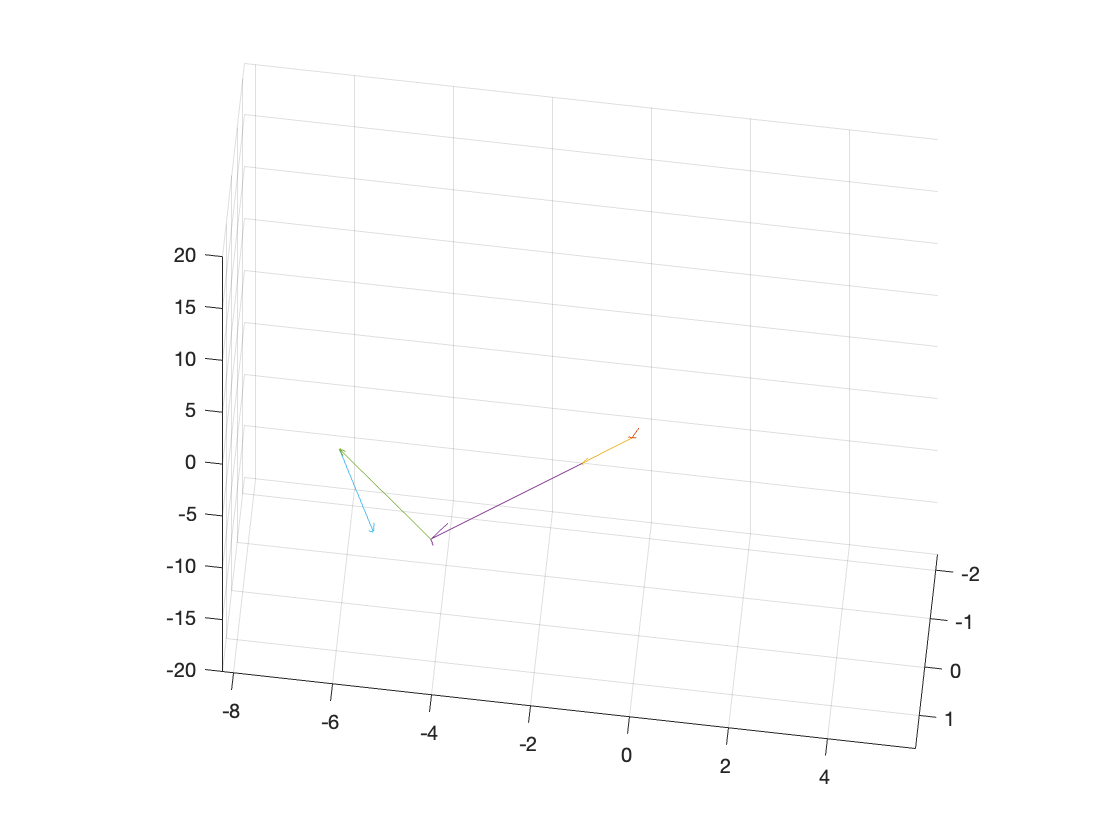
\includegraphics[scale=0.3]{fig1.png}
    \caption{Path of Newton's Method}
    \label{fig:my_label}
\end{figure}
\section*{Problem \#4}
Here we will use the calculus approach for finding the critical points of $f(x)$, that is by first setting the gradient to $0$ to obtain,

\begin{equation*}
    \begin{cases}
        8x_1^3-4x_2 &= 0 \\
        2x_2-4x_1 + 5 &= 0
    \end{cases}
\end{equation*}
and get
\begin{align*}
    x_1 &= -1.38041 \\
    x_2 &= -5.26082
\end{align*}
as the only real-valued critical point. 

Note that the Hessian evaluated at this point is,

\begin{equation*}
    Hf(x_1,x_2) = \begin{bmatrix*}[r]45.7327 & -4 \\ -4 & 2\end{bmatrix*}
\end{equation*}

which is Positive Definite, thus $(x_1,x_2)$ is a local minimum. We can extend this to show that $(x_1,x_2)$ is also a global minimum as well.

\section*{Problem \#5}

\begin{figure}[H]
    \centering
    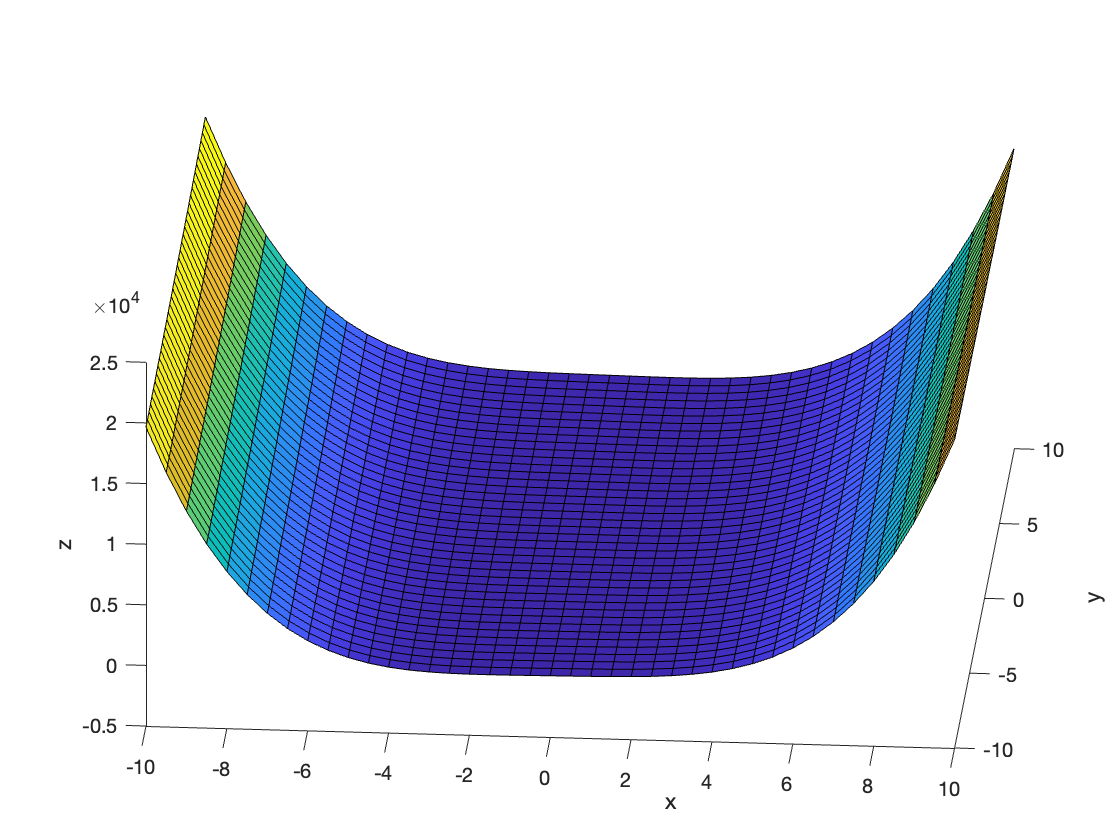
\includegraphics[scale=0.3]{fig2.png}
    \caption{Plot of $f(x)$}
    \label{fig:my_label}
\end{figure}

\begin{figure}[H]
    \centering
    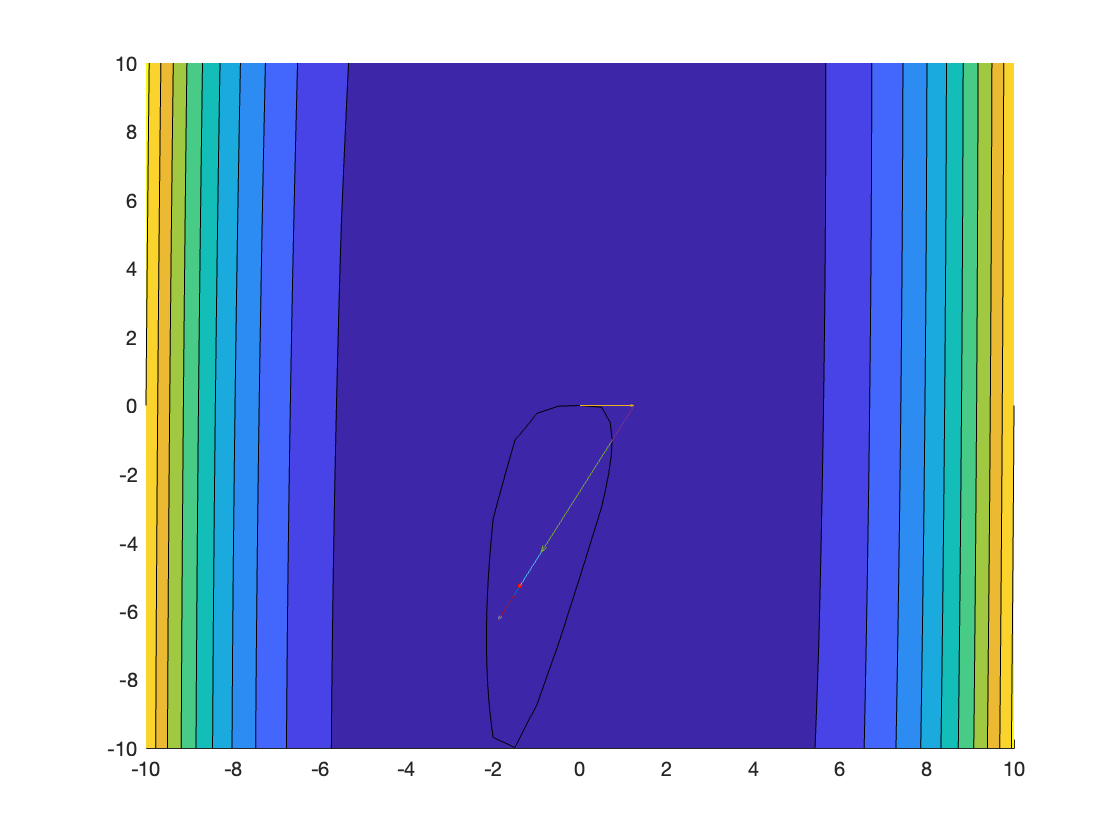
\includegraphics[scale=0.3]{fig3.png}
    \caption{Contour Plot of $f(x)$}
    \label{fig:my_label}
\end{figure}
\end{document}